\begin{titlingpage}
\begin{center}
\vspace*{1in}

\textbf{\large CS221: Digital Design}


\bigskip

\vspace*{1in}

Waleed A. Yousef, Ph.D.,

\bigskip

Human Computer Interaction Lab.,\\Computer Science Department,\\Faculty of Computers and Information,\\Helwan University,\\Egypt.

\bigskip

\today

\end{center}
\end{titlingpage}


\textbf{Lectures follow (and some figures are adapted from):}

\bigskip

\begin{window}[0,1,{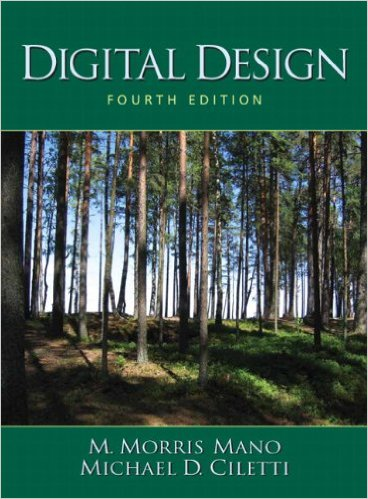
\includegraphics[width=.3\textheight]{FrontMatter/Mano.jpg}},{}]
\bibentry{Mano2007DigDes}
\end{window}



\vspace{2.5in}

\textbf{We will proceed as follows:}

\begin{itemize}
  \item Fast introduction (few sections from Chapter 1).

  \item Detailed study of Chapters 2-7; very few sections will be
  skipped. At the end of each chapter Verilog code for some circuits
  will be explained.

  \item If time permits, Chapter 8 will be covered in full or in parts
\end{itemize}

\clearpage

\chapter*{Course Objectives}
This course combines three approaches to teach students Digital
Design, which is the fundamental prerequisite to understand computer design and architecture:


\begin{enumerate}
  \item Theoretical aspects of the subject will be covered in
  lectures, along with exercises in sections. Students, by the end of
  the course, should be able to design, analyze, and implement
  combinational and synchronous digital circuits.

  \item A second objective is to teach students the digital design
  using a Hardware Descriptive Language (HDL). Students by the end of
  the semester will be able to analyze logic circuits with Verilog
  (one of the available HDLs).

  \item A third objective is to develop the practical sense of the
  students through lab. experiments. Students will be able to
  implement logic circuits using breadboards and ICs.
\end{enumerate}

\clearpage
{
\tiny
\settocdepth{subsection}
\tableofcontents
}


%%% Local Variables:
%%% mode: latex
%%% TeX-master: "../LectureNotesCS221"
%%% End:
